\documentclass[11pt,a4paper]{article}
\usepackage[utf8]{inputenc}
\usepackage[hmargin=2.0cm,vmargin=2.5cm,bindingoffset=0.5cm]{geometry}
\usepackage{amsfonts}
\usepackage{amsmath,amsthm,amssymb}
\usepackage{hyperref}
\usepackage{graphicx}
\usepackage{tikz}
\usepackage{mathtools}
\DeclarePairedDelimiter\ceil{\lceil}{\rceil}
\DeclarePairedDelimiter\floor{\lfloor}{\rfloor}
%\usepackage{float}
\usepackage{placeins}
\usepackage{diagbox}
\newtheorem{thm}{Theorem}
\usepackage{subcaption}
%\usepackage{subfigure}
\usepackage[english]{babel}
\author{Mohit}
\title{Counterdiabatic driving}
\begin{document}
\maketitle

\section{Goal}

The goal, as of now, is to distinguish between integrable and non-integrable many-body quantum system by studying their approximate gauge adiabatic potential\footnote{We expect results to be valid for classical system too. But for now, we would focus on quantum systems.}

 
Classically, on one hand, integrable systems have a lot of constants of motion, and as a result, they have a few independent degrees of freedom. On the other hand, non-integrable systems contain a large number of independent degrees of freedom. We expect a similar picture for quantum systems.

The central idea is to apply Eigenstate Thermalization Hypothesis (ETH) to operators of approximate gauge potential in non-integrable quantum systems, and claim that its' norm scales exponentially in system 
size. Whereas for integrable systems, approximate gauge potential are supposed to scale like a polynomial in system size.

\section{Introduction}
\subsection{Integrable and non-integrable systems}
What is an integrable quantum systems? To the best of my knowledge, the general definition of integrability for quantum systems has not been reached conclusively. Despite this, there are some models which are commonly agreed to be integrable and similarly, there are model which are called non-integrable in literature. For our purposes, we would use such models to get some intuition.

Let's list down a few properties of \textbf{integrable} quantum systems: 
\begin{itemize}
\item Density of those systems don't thermalize to Gibbs distribution. In fact, they thermalize to a generalized Gibbs distribution. (see Rigol papers for detail) 
\item They can be diagonalized using a transformation that is local in space\footnote{According to Dries, for 2D transverse quantum Ising model, Jordan Wigner transformation exists to diagonalize the Hamiltonian. However, it's still called a non-integrable model since then the transformation becomes non-local. I need to dig relevant paper for details}. Examples are non-interacting fermions, 1 D Ising model and 1D transverse field Ising model (TFIM).  These can be diagonalized using Bogoliubov, transfer matrix method and Jordan-Wigner transformation, respectively.
\item ETH doesn't apply to them (cite relevant papers)
\item Distribution of Energy level spacing follows Poisson distribution --energy level attraction.
\end{itemize}


Let's list down a few properties of \textbf{non-integrable} quantum systems: 
\begin{itemize}
\item Density of those systems thermalize to Gibbs distribution.  (see Rigol papers for detail) 
\item They cannot be diagonalized using a transformation that is local in space. This is not a strong argument because it just means that such a transformation has not been found yet.
\item ETH does apply to them (cite relevant papers)
\item Distribution of Energy level spacing are correlated and therefore, they show level repulsion. They follow Wigner-Dyson or similar distributions, depending upon the details of Hamiltonian. These properties can be derived using Random Matrix Theory.
\end{itemize}


We do note that both integrable and non-integrable show quantum phase transition \footnote{Is there any difference between phase transitions shown between integrable and non-integrable models? Apparently no.}. An example of quantum phase transition in integrable model: TFIM show paramagnetic-ferromagnetic quantum phase transition.

\subsection{What are adiabatic gauge potentials?}
\subsubsection*{Gauge potential}
Let's represent a wavefunction in some basis:
\begin{equation}
|\psi \rangle= \sum_n \psi_n |n \rangle_0
\end{equation}
where $|n \rangle_0$ is some fixed, parameter independent basis. Now let's do a unitary basis transformation to $|m (\lambda) \rangle$ in the parameter $\lambda$ dependent space using $U(\lambda)$:
\begin{equation}
|m (\lambda) \rangle= \sum_n U_{mn} |n \rangle
\end{equation}
Hence, now we can express $|\psi \rangle = \sum_m \tilde{\psi_n}  |m (\lambda) \rangle $, where $\tilde{\psi_n}= \langle  m (\lambda) |\psi \rangle $
 
Quantum gauge potentials are defined to be generators of continuous unitary transformation.
$A_{\lambda}= i \hbar \partial_{\lambda}$. Here I am listing some properties:
\begin{itemize}
\item They are Hermitian operator.\
\item $\langle n (\lambda)| A_{\lambda}| m(\lambda) \rangle = {}_0\langle  n| A_{\lambda}| m(\lambda) \rangle_0$
\end{itemize}
 

\subsubsection*{Adiabatic gauge potential}
The gauge potentials become adiabatic gauge potential when unitary transformation generated by $A_{\lambda}$ are used to diagonalize Hamiltonian.

 Adiabatic gauge potentials are a special subset of these which diagonalize  the instantaneous Hamiltonian, attempting to leave its eigenbasis invariant as the parameter is changed. These adiabatic gauge potentials generate non-adiabatic corrections to Hamiltonian in the moving basis.
 
 This is something from Anatoli's lecture notes--
``an adiabatic basis as a family of adiabatically connected eigenstates, i.e., eigenstates related
to a particular initial basis by adiabatic (infinitesimally slow) evolution of the parameter $\lambda$. For example, if two levels cross they will exchange order energetically but the adiabatic connection will be non-singular."


$H (\lambda) |n(\lambda) \rangle = E_n (\lambda) |n(\lambda) $. Let's derive diagonal and off-diagonal elements. 

\begin{itemize}
\item \textbf{n-th diagonal element:} $A_{\lambda}^n= \langle n |A_{\lambda} | n \rangle= \langle n |\partial_{\lambda} | n \rangle $
\item \textbf{off- diagonal element:} We use the identity $\langle m |H(\lambda) | n \rangle=0 \quad, n \neq m$ and then differentiate with respect to $\lambda$ to obtain:
\begin{align}
\langle m |A_{\lambda} | n \rangle = i \hbar \dfrac{\langle n |\partial_{\lambda}H | n \rangle}{E_m-E_n}
\end{align}

\end{itemize}


\section{Adiabatic gauge potential}
Our Hamiltonian would be controlled using a control parameter called $\lambda$. Our aim would be drive the system without any transition.

Let Hamiltonian $H_0(\lambda (t))$ satisfy the following equation

\begin{equation}
H_0(\lambda (t)) |\psi \rangle= i \partial_t|\psi \rangle
\end{equation}

Let us go to rotating frame so as to diagonalize our Hamiltonian. Required unitary transformation $U(\lambda)$ would depend on parameter $\lambda$. Wave function in moving frame is $|\tilde{\psi}  \rangle = U^{\dagger} |\tilde{\psi}  \rangle$. In this basis, Hamiltonian is diagonal:
$\tilde{H_0}= U^{\dagger} H_0 U = \sum_n \epsilon (\lambda)  |n (\lambda)\rangle \langle  n (\lambda) |$. \footnote{Note that expectation value should remain same in both basis, i.e.$ \langle \tilde{\psi} | \tilde{H_0}  |\tilde{\psi}  \rangle= \langle{\psi} | {H_0}  |{\psi}  \rangle$}

How does the wave function evolve in new basis?
\begin{equation}
 i \partial_t|\tilde{\psi} \rangle=(\tilde{H_0
 }(\lambda (t)) - \dot{\lambda} \tilde{\mathcal{A_\lambda}}) |\psi \rangle
\end{equation}

Note that gauge potential should be purely imaginary. But this doesn't mean that it has to be necessarily anti-Hermitian for a real Hamiltonian.

$\clubsuit \clubsuit $Things to include here \\
Derive the commutator relation, write the variational approach.

\section{Our model: spin chain with transverse and longitudinal field}

\begin{equation}
H_0=\sum_{j=1}^{L-1} J(\lambda) \sigma_j^z \sigma_{j+1}^z + \sum_{j=1}^{L}  (Z_j (\lambda) \sigma_j^z +X_j (\lambda) \sigma_j^x)
\end{equation}

We note that for either $Z_j=0$ or $X_j=0$, this model is integrable. Apart from these cases, this model is non-integrable. \footnote{David Huse and Kim have mentioned in their paper which parameter are best for the spin chain to be integrable. Since our method also depends on exact diagonalization, I should use their results.}


Here we would try to reproduce figure 4 of Dries paper.

\begin{equation}
H_0=\sum_{j=1}^{L-1}  \sigma_j^z \sigma_{j+1}^z + \sum_{j=1}^{L} (2\sigma_j^z + 0.8 \sigma_j^x ) + \lambda \sigma_0^x
\end{equation}
\begin{equation}
\lambda(t) = \lambda_0 + (\lambda_f-\lambda_0)\sin\left(\dfrac{\pi}{2}\left(\sin(\dfrac{t\pi}{2.0 \tau})^2 \right) \right)^2 \quad, t \in [0, \tau]
\end{equation}
\begin{figure}
\centering
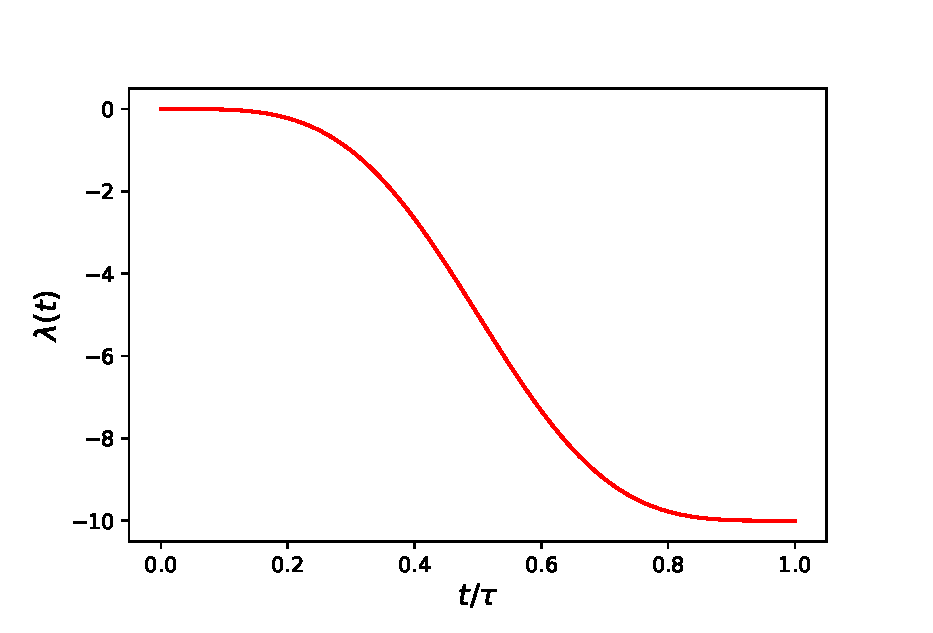
\includegraphics[scale=0.67]{protocol.eps}
\caption{Protocol chosen for going from $\lambda_i=0$ to $\lambda_i=1$ in time $\tau$}
\end{figure}

$\clubsuit \clubsuit $Things to include here \\


\begin{figure}
\centering
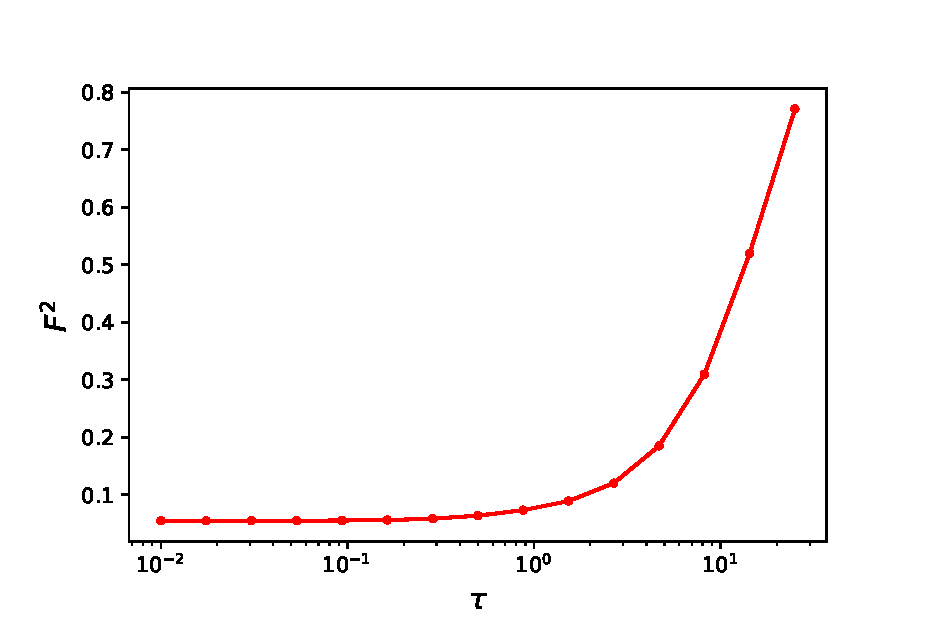
\includegraphics[scale=0.5]{fidelity_naive.eps}
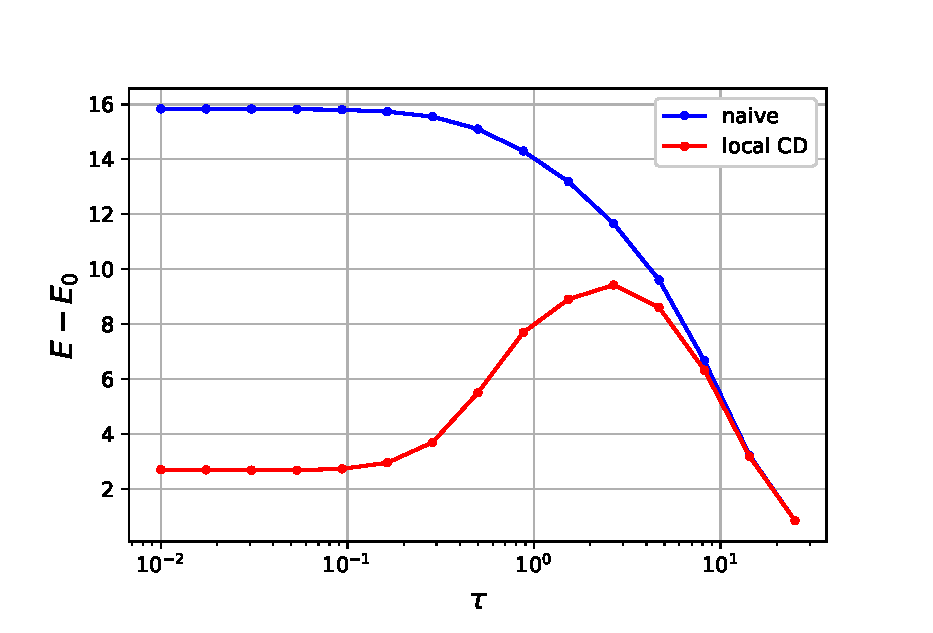
\includegraphics[scale=0.5]{final_energy_naive.eps}
\caption{Fidelity and final energy above ground state}
\end{figure}

CD Hamiltonian $H_0+ \lambda \sigma_0^x + \dot{\lambda} \alpha_0 \sigma_0^y$\\
\appendix

\section{Spin 1/2 particle in a time-dependent magnetic field}
I would include a derivation from lecture notes to gain an intuition here. I also plan to understand Berry's paper and reproduce some of his calculations in this appendix.

\section{Free interacting fermions in an external potential}

\begin{equation}
H_0= -J \sum_{j=1}^{L-1} (c^{\dagger}_j c_{j+1} +c^{\dagger}_{j+1} c_{j}) + \sum_{j=1}^{L} V_j(\lambda) c^{\dagger}_jc_j
\end{equation}


\begin{equation}
\mathcal{A}^*_{\lambda}= i  \sum_{j=1}^{L-1} \alpha_j (c^{\dagger}_j c_{j+1} - c^{\dagger}_{j+1} c_{j}) 
\end{equation}

include pictures drawn using sympy


\section{Classical adiabatic gauge potential}
Let's start by considering classical systems. For such systems, we specify the system by defining Hamiltonian $H (\lambda)$ in terms of canonical variables $q_i (\lambda,t)$ and $p_j (\lambda,t)$. where $\lambda$ is an externally controlled parameter. These variables satisfy the canonical relations:
\begin{equation}
\{q_i,p_j \}=\delta_{ij} 
\end{equation}
where $\{\ldots \}$ denotes the Poisson bracket.

Canonical transformations are transformations of $q_i$ and $p_j$ to new variables $\bar{q_i}$ and $\bar{p_j}$ such that it preserves Poisson bracket. Hence, 
\begin{equation}
\{\bar{q_i},\bar{p_j} \}=\delta_{ij} 
\end{equation}

What are gauge potentials? Gauge potential $A_{\lambda}$  are the generators of continuous canonical transformations in parameter $\lambda$ space , which can be defined as :
\begin{alignat}{5}
q_j(\lambda + \delta \lambda) & =& q_j - \dfrac{\partial A_{\lambda}}{\partial p_j} \delta \lambda &\Rightarrow & \dfrac{\partial q_j}{\partial \lambda} &=& -\dfrac{\partial A_{\lambda}}{\partial p_j} = \{A_{\lambda},q_j \} \\
p_j(\lambda + \delta \lambda) & =& p_j + \dfrac{\partial A_{\lambda}}{\partial q_j} \delta \lambda & \Rightarrow & \dfrac{\partial p_j}{\partial \lambda} &=& \dfrac{\partial A_{\lambda}}{\partial q_j}=\{ A_{\lambda},p_j \}
\label{def_A}
\end{alignat}

We can verify that these transformations are canonical upto order $\delta \lambda ^2$ because we can show that:
\begin{equation}
\{q_j(\lambda + \delta \lambda), p_j(\lambda + \delta \lambda)\} = \delta_{ij} + O(\delta \lambda ^2)
\end{equation}

Let's try to understand by taking an example of continuous canonical transformation. We would shift the position coordinate by $X_i$. Here our parameter $\lambda$ is $X_i$
\begin{eqnarray}
 q_i(X_i,t) &=& q_i(0,t) - X_i \\
p_i(X_i,t)&=& p_i(0,t)
\end{eqnarray}
Using equation \ref{def_A}, we see that $\frac{\partial A_{X_i}}{\partial q_j}=0$ and $-\frac{\partial A_{X_i}}{\partial p_j}=-\delta_{ij}$. Hence, $A_{X_i}=p_j + C_j$, where $C_j$ are arbitrary constants of integration. This is the gauge choice we have got in defining these gauge potentials. 



\end{document}